\documentclass[11pt,letterpaper]{article}

\usepackage[utf8]{inputenc}
\usepackage[T1]{fontenc}
\usepackage[spanish,es-nodecimaldot]{babel}
\usepackage{lmodern}
\usepackage{microtype}
\usepackage[margin=2.5cm,headheight=14pt]{geometry}
\usepackage{graphicx}
\usepackage{booktabs}
\usepackage{tabularx}
\usepackage{longtable}
\usepackage{array}
\usepackage{amsmath}
\usepackage{xcolor}
\usepackage{enumitem}
\usepackage{caption}
\usepackage{float}
\usepackage{fancyhdr}
\usepackage{hyperref}

\definecolor{uvgblue}{HTML}{17365D}
\definecolor{lightblue}{HTML}{EAF1F8}
\hypersetup{
  colorlinks=true,
  linkcolor=uvgblue,
  citecolor=uvgblue,
  urlcolor=uvgblue,
  pdftitle={Laboratorio 5: Clasificación de tweets usando minería de texto},
  pdfsubject={CC3084 Data Science},
  pdfauthor={Anggie Quezada, Iris Ayala y Jonathan Díaz}
}
\setlength{\parindent}{0pt}
\setlength{\parskip}{0.55em}
\setlist{itemsep=0.2em,topsep=0.3em}
\renewcommand{\arraystretch}{1.18}
\captionsetup{font=small,labelfont=bf}
\emergencystretch=2em

\pagestyle{fancy}
\fancyhf{}
\lhead{CC3084 --- Data Science}
\rhead{Laboratorio 5}
\cfoot{\thepage}

\newcommand{\code}[1]{\texttt{#1}}
\newcolumntype{Y}{>{\raggedright\arraybackslash}X}
\newcolumntype{C}[1]{>{\centering\arraybackslash}p{#1}}

\begin{document}
\pagenumbering{gobble}

\begin{titlepage}
  \centering
  {\Large\bfseries Universidad del Valle de Guatemala\par}
  \vspace{0.35cm}
  {\large Facultad de Ingeniería\par}
  {\large Departamento de Ciencias de la Computación\par}
  \vspace{1.2cm}
  {\large CC3084 --- Data Science\par}
  {\large Semestre II, 2026\par}
  \vfill
  {\color{uvgblue}\rule{\textwidth}{1.2pt}\par}
  \vspace{0.45cm}
  {\Huge\bfseries Laboratorio 5\par}
  \vspace{0.25cm}
  {\LARGE Clasificación de tweets usando minería de texto\par}
  \vspace{0.45cm}
  {\color{uvgblue}\rule{\textwidth}{1.2pt}\par}
  \vfill
  \fbox{\begin{minipage}{0.82\textwidth}
    \centering
    \textbf{Integrantes del grupo}\par
    \vspace{0.35cm}
    \textbf{Anggie Quezada}\par
    \textbf{Iris Ayala}\par
    \textbf{Jonathan Díaz}\par
  \end{minipage}}
  \vfill
  {\large 29 de agosto de 2026\par}
  \vspace{0.45cm}
  {\small Informe y repositorio: \url{https://github.com/Qu3zada22/lab5-ds}\par}
\end{titlepage}

\pagenumbering{roman}
\begingroup
\small
\setlength{\parskip}{0pt}
\tableofcontents
\endgroup
\clearpage
\pagenumbering{arabic}

\section{Introducción}

Se construyó un flujo reproducible para clasificar tweets en inglés como referencias a un desastre real (\code{target=1}) o usos no literales y conversaciones ordinarias (\code{target=0}). El análisis supervisado utiliza los 7,613 registros de entrenamiento de la competencia de Kaggle. Se normalizó el texto para el análisis temático, se estudiaron frecuencias y n-gramas dentro de cada tweet, y se compararon Naive Bayes multinomial, regresión logística y una máquina de soporte vectorial lineal sobre TF--IDF de unigramas y bigramas.

La regresión logística obtuvo el mejor equilibrio en prueba: exactitud 0.822718 y F1 0.776490. El análisis de sentimiento se realizó separadamente sobre el texto original mediante VADER, para conservar puntuación, mayúsculas y emoticones. Los tweets de desastre presentaron una negatividad media mayor (0.173582 frente a 0.132318), pero el efecto rango-biserial fue pequeño (0.1465). Agregar la negatividad como característica no mejoró el clasificador: el F1 disminuyó a 0.775104 ($\Delta=-0.001386$). En consecuencia, el producto final conserva la regresión logística basada exclusivamente en TF--IDF.

\section{Objetivo}

El objetivo general fue desarrollar y evaluar un sistema reproducible que reciba un tweet sin preprocesar y determine si describe un desastre real. Para ello se buscó: (i) comprender la calidad, balance y vocabulario del conjunto; (ii) documentar la limpieza; (iii) estudiar unigramas, bigramas y trigramas; (iv) comparar clasificadores mediante métricas apropiadas; (v) analizar sentimiento y negatividad; y (vi) comprobar empíricamente si la negatividad aporta señal predictiva adicional.

\section{Datos y alcance del análisis}

\subsection{Origen y tamaño}

Los datos proceden de la competencia \emph{Natural Language Processing with Disaster Tweets} de Kaggle \cite{kaggle}. La consigna indica ``más de 10,500 filas'' porque la entrega de Kaggle comprende 7,613 filas etiquetadas en \code{train.csv} y 3,263 filas sin etiqueta en \code{test.csv}, es decir, 10,876 registros en conjunto. El presente análisis supervisado usa únicamente \code{train.csv}, porque es el archivo que contiene la variable objetivo y el solicitado expresamente para entrenamiento y evaluación.

\begin{table}[H]
\centering
\caption{Variables del conjunto de entrenamiento.}
\label{tab:variables}
\begin{tabularx}{\textwidth}{@{}lYl@{}}
\toprule
Variable & Descripción & Tipo observado \\
\midrule
\code{id} & Identificador del tweet. & Entero \\
\code{keyword} & Palabra clave asociada; puede estar ausente. & Texto \\
\code{location} & Ubicación declarada por el usuario; puede estar ausente y no está normalizada. & Texto \\
\code{text} & Contenido original del tweet. & Texto \\
\code{target} & Clase: 1 para desastre real y 0 para no desastre. & Entero binario \\
\bottomrule
\end{tabularx}
\end{table}

\subsection{Balance y valores ausentes}

El conjunto presenta un desbalance moderado, no extremo: 4,342 tweets no asociados con desastres y 3,271 asociados con desastres. Por ello se usó estratificación y se priorizó F1, sin limitar la evaluación a exactitud.

\begin{table}[H]
\centering
\caption{Distribución de la variable objetivo.}
\label{tab:balance}
\begin{tabular}{@{}lrr@{}}
\toprule
Categoría & Frecuencia & Porcentaje \\
\midrule
No desastre (0) & 4,342 & 57.03\% \\
Desastre real (1) & 3,271 & 42.97\% \\
\midrule
Total & 7,613 & 100.00\% \\
\bottomrule
\end{tabular}
\end{table}

No existen nulos en \code{text}, \code{target} ni \code{id}. \code{keyword} tiene 61 ausencias (0.80\%) y \code{location}, 2,533 (33.27\%). La segunda variable es además texto libre y heterogéneo, por lo que no se imputó ni incorporó al modelo principal. Esta exclusión evita imponer una interpretación geográfica falsa, aunque también deja señal potencial sin explorar.

\section{Metodología reproducible}

El trabajo se ejecutó con \code{uv 0.11.28}, Python 3.9.25 y JupyterLab. El entorno bloqueado contiene pandas 2.3.3, NumPy 2.0.2, scikit-learn 1.6.1, SciPy 1.13.1, NLTK 3.9.2, Matplotlib 3.9.4 y wordcloud 1.9.6. Las restricciones directas están declaradas en \code{pyproject.toml} y la resolución exacta en \code{uv.lock}.

El protocolo experimental fue el siguiente:
\begin{enumerate}
  \item cargar los 7,613 registros etiquetados y auditar esquema, nulos y balance;
  \item construir \code{text\_cleaned} para análisis léxico y clasificación temática;
  \item separar una sola vez 80\% para entrenamiento (6,090 tweets) y 20\% para prueba (1,523), con \code{random\_state=42} y \code{stratify=y};
  \item ajustar TF--IDF únicamente sobre entrenamiento, con unigramas y bigramas y un máximo de 5,000 características;
  \item entrenar y comparar tres clasificadores sobre exactamente el mismo split;
  \item calcular VADER sobre \code{text} original y reutilizar los mismos índices para evaluar la característica \code{negativity}, sin reajustar TF--IDF con prueba.
\end{enumerate}

Las nubes de palabras usan también semilla 42. El notebook descargó de NLTK los recursos \code{stopwords} y \code{vader\_lexicon} cuando no estaban disponibles. Los comandos completos se incluyen en el anexo de reproducibilidad.

\section{Limpieza y preprocesamiento}

\subsection{Texto para clasificación temática}

La función \code{limpiar\_tweet} aplica las transformaciones en un orden fijo:
\begin{enumerate}
  \item convierte a minúsculas;
  \item elimina URLs con expresiones regulares;
  \item elimina menciones completas de la forma \code{@usuario};
  \item elimina el símbolo \code{\#}, pero conserva la palabra del hashtag;
  \item elimina todos los dígitos;
  \item conserva solo letras inglesas y espacios, con lo cual elimina puntuación, apóstrofes, caracteres especiales y emoticones;
  \item normaliza espacios y elimina las \emph{stopwords} inglesas de NLTK.
\end{enumerate}

La decisión sobre números es deliberadamente simplificadora: la expresión \code{\textbackslash d+} elimina también \code{911}. Esto reduce variantes y ruido, pero puede descartar una señal relevante de emergencia; debe considerarse una limitación y una hipótesis para trabajo posterior. Ningún registro quedó vacío. Por ejemplo, ``Our Deeds are the Reason of this \#earthquake May ALLAH Forgive us all'' se transforma en ``deeds reason earthquake may allah forgive us''.

\subsection{Texto para sentimiento}

La limpieza temática no se reutilizó para VADER. El sentimiento se calculó sobre \code{text} original porque VADER fue diseñado para redes sociales y sus reglas consideran mayúsculas, signos de exclamación, puntuación, negaciones, intensificadores y emoticones \cite{hutto2014,nltkvader}. Esta separación evita destruir información afectiva al mismo tiempo que mantiene una representación temática más compacta para TF--IDF.

\section{Análisis exploratorio}

\subsection{Frecuencias y vocabulario compartido}

En desastres, las palabras más frecuentes incluyen \emph{fire} (180), \emph{news} (138), \emph{disaster} (117), \emph{california} (111), \emph{suicide} (110), \emph{killed} (93) y \emph{storm} (85). En no desastres destacan \emph{like} (253), \emph{im} (248), \emph{amp} (193), \emph{new} (170), \emph{get} (163), \emph{dont} (154) y \emph{love} (90). La Figura~\ref{fig:frecuencias} hace visible la diferencia entre términos de eventos concretos y lenguaje conversacional.

\begin{figure}[H]
  \centering
  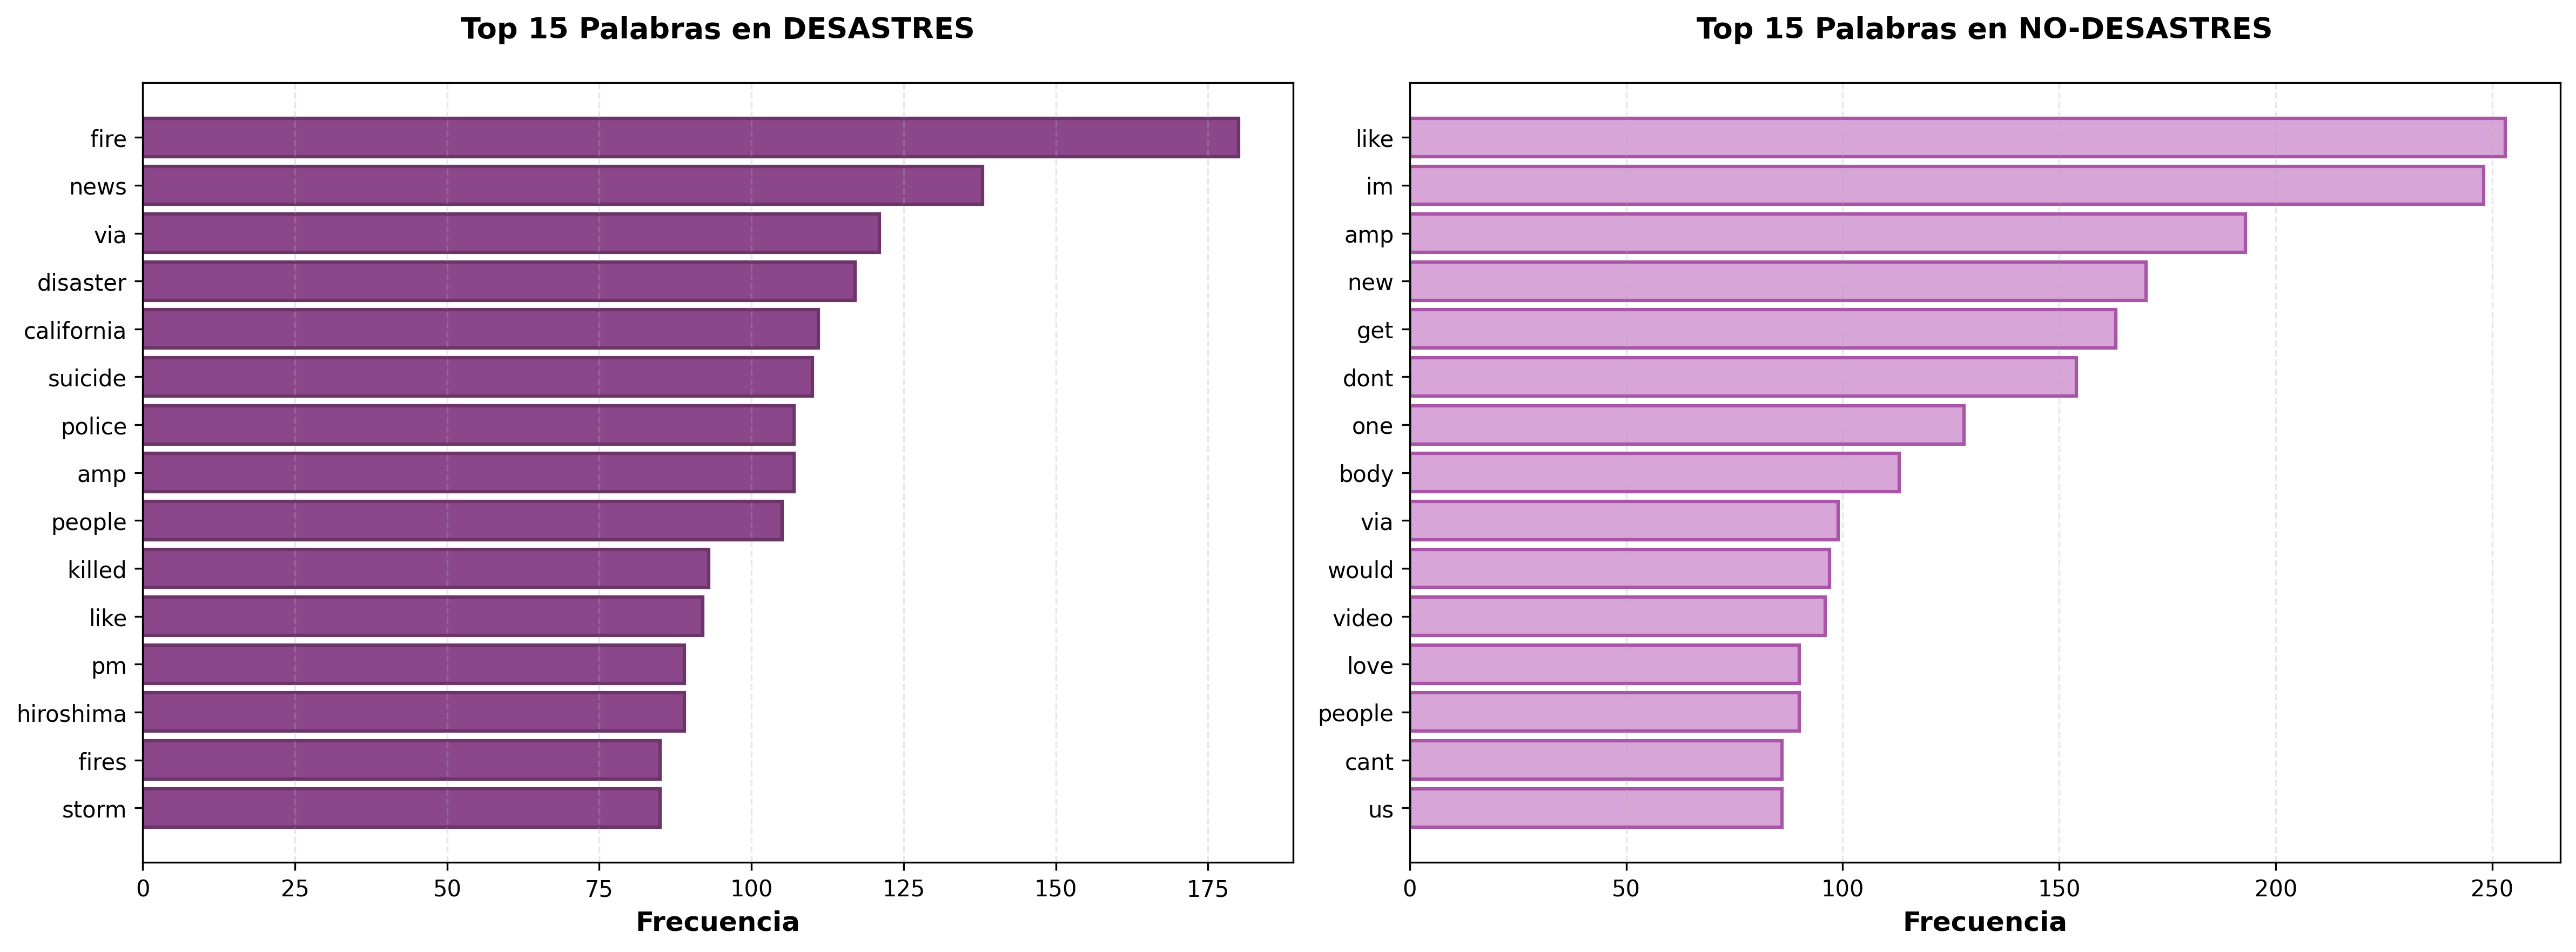
\includegraphics[width=\textwidth]{../img/frecuencia_palabras_comparacion.png}
  \caption{Quince palabras más frecuentes en tweets de desastres y no desastres.}
  \label{fig:frecuencias}
\end{figure}

Palabras como \emph{via}, \emph{amp}, \emph{people} y \emph{like} aparecen en ambas clases; una frecuencia alta aislada no basta para discriminar. En contraste, ratios exploratorios suavizados identificaron términos muy inclinados hacia desastres, como \emph{northern}, \emph{legionnaires}, \emph{debris}, \emph{severe} e \emph{hiroshima}, y hacia no desastres, como \emph{bags}, \emph{bag}, \emph{aftershock}, \emph{ruin} y \emph{lmao}. Algunos reflejan eventos o usos metafóricos específicos, por lo que no deben interpretarse como relaciones causales.

El vocabulario contiene 8,006 tipos en desastres y 10,372 en no desastres. Solo 3,805 aparecen en ambas clases; 4,201 son exclusivos del primer grupo y 6,567 del segundo. La Figura~\ref{fig:vocabulario} resume este solapamiento. Aunque sugiere separabilidad léxica, muchos tipos exclusivos son errores tipográficos, nombres propios o fragmentos poco frecuentes.

\begin{figure}[H]
  \centering
  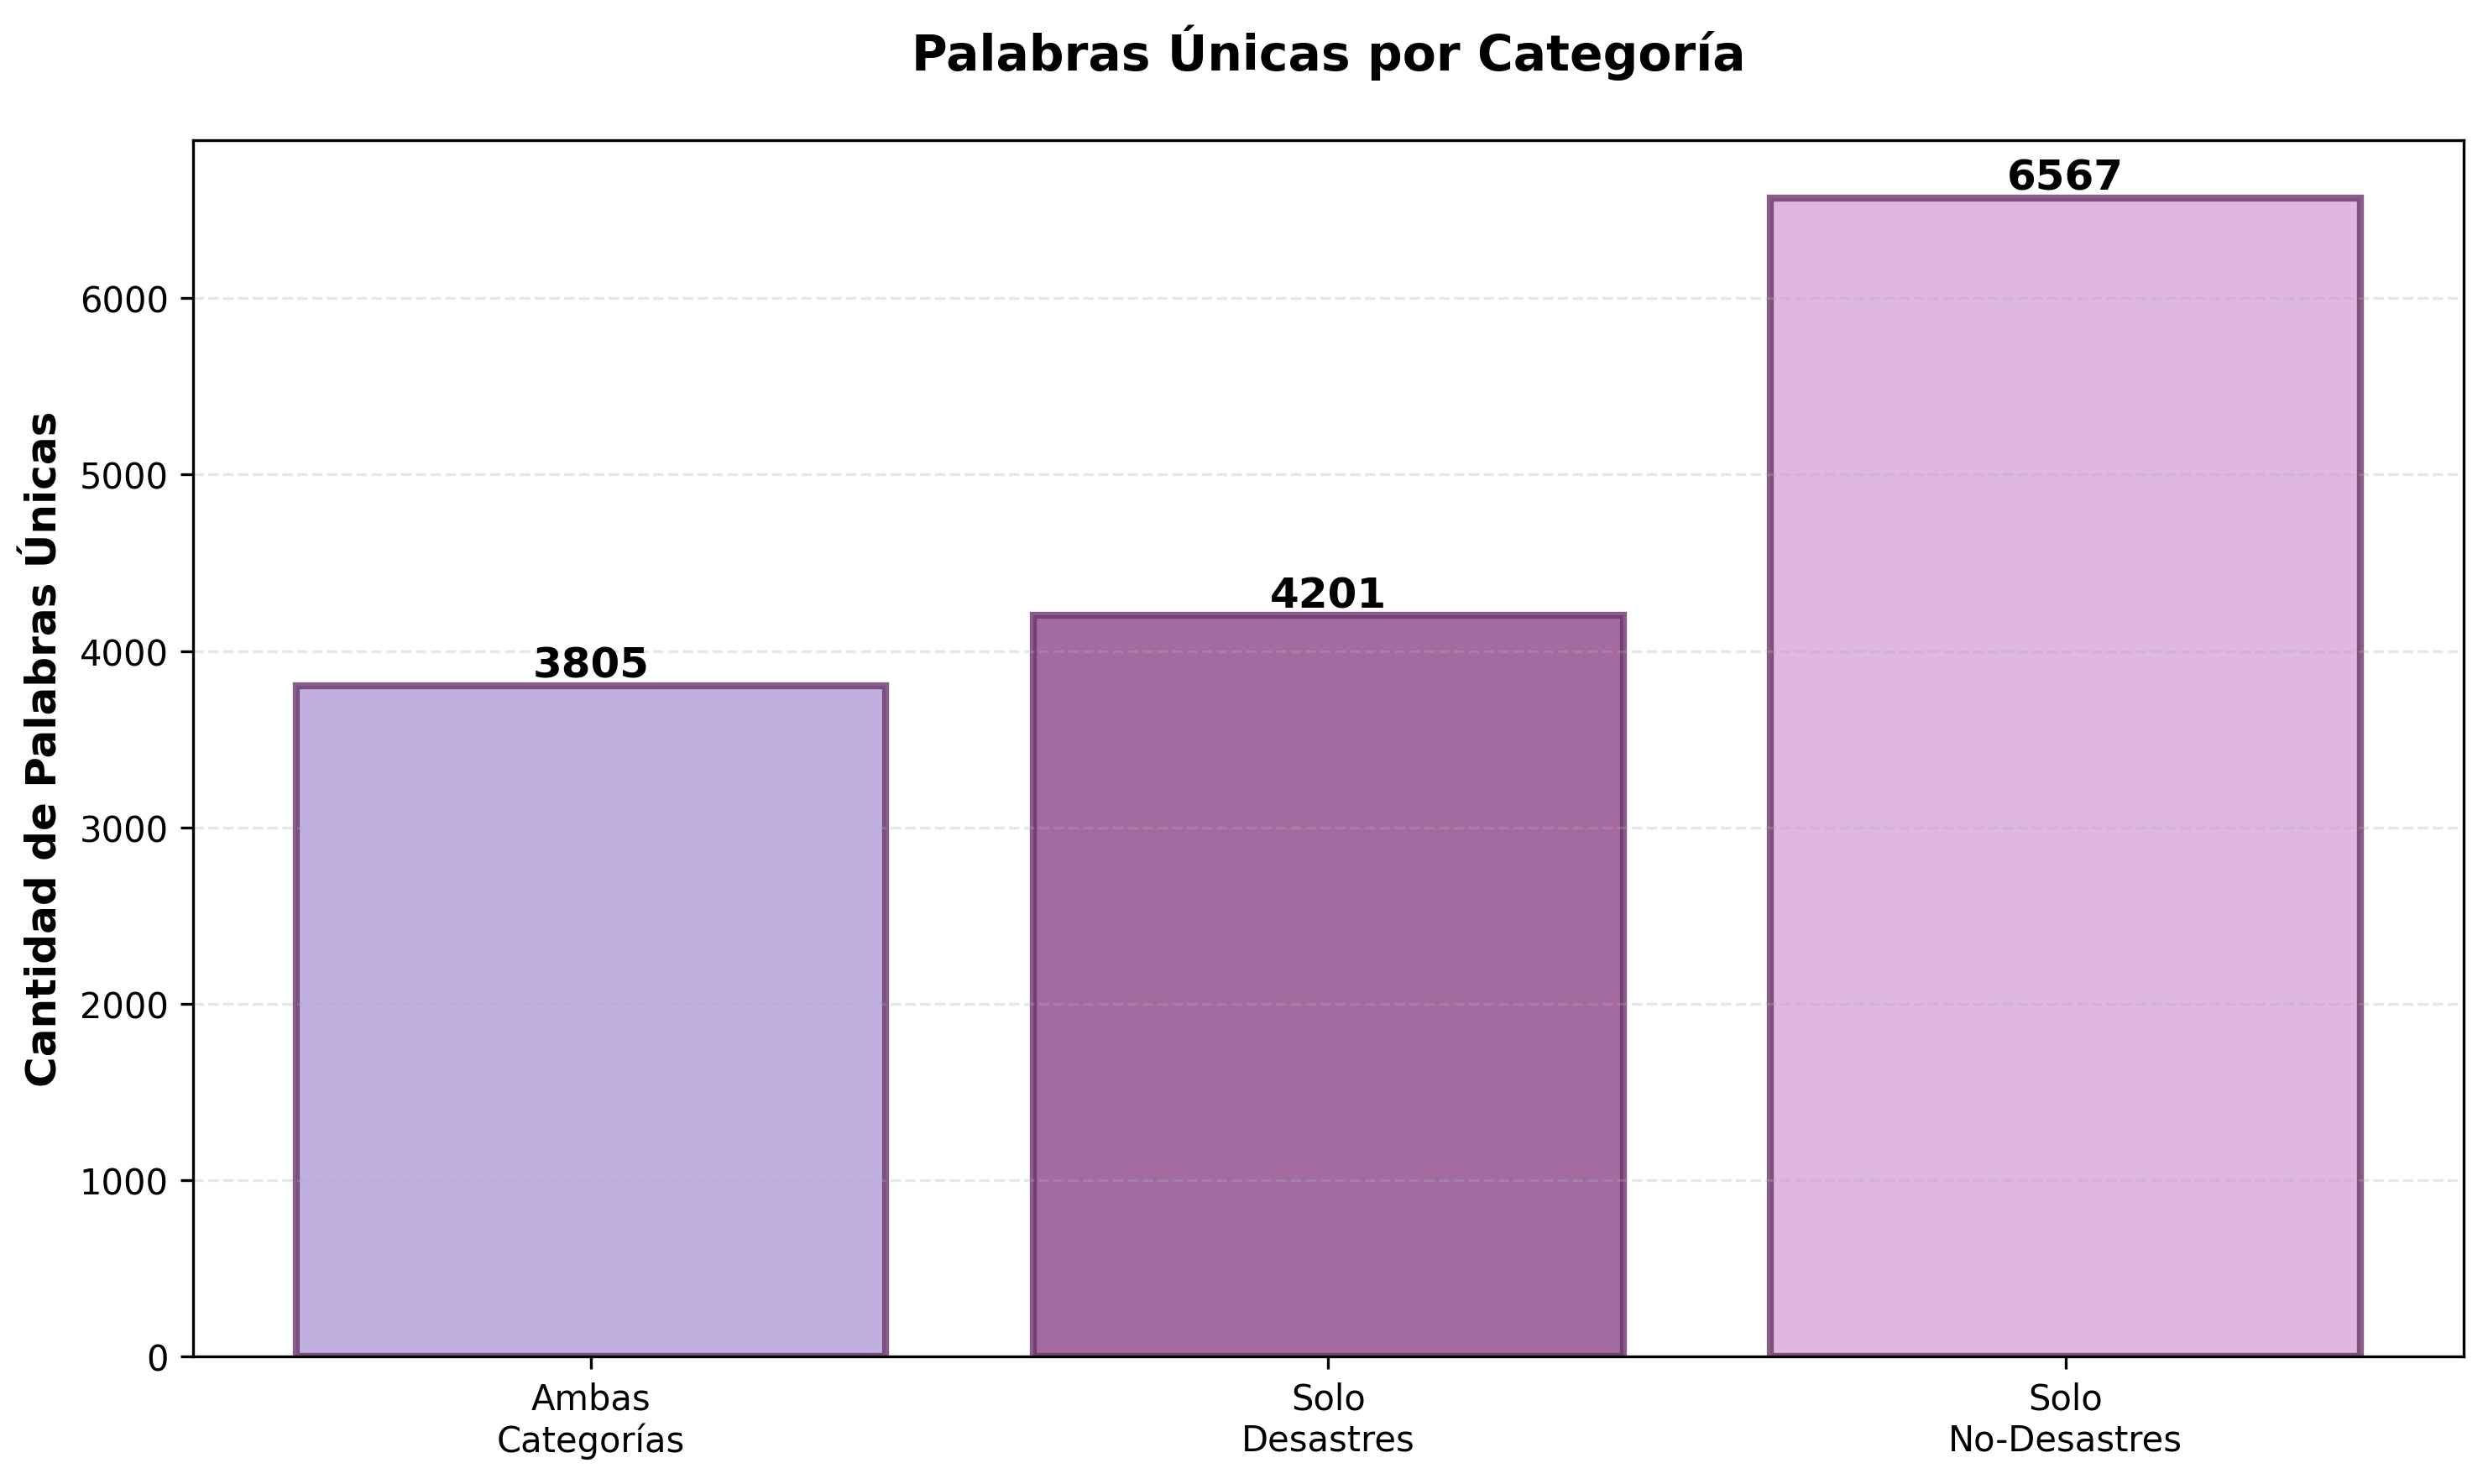
\includegraphics[width=0.78\textwidth]{../img/palabras_analisis.png}
  \caption{Cantidad de palabras compartidas y exclusivas por categoría.}
  \label{fig:vocabulario}
\end{figure}

\subsection{Nubes de palabras}

Las nubes de la Figura~\ref{fig:nubes} corroboran el patrón: la clase de desastre está dominada por vocabulario de emergencia, noticias, lugares e incidentes; la clase no desastre contiene más lenguaje cotidiano y afectivo. Estas visualizaciones resumen frecuencia, pero no corrigen por tamaño de clase ni prueban capacidad predictiva.

\begin{figure}[H]
  \centering
  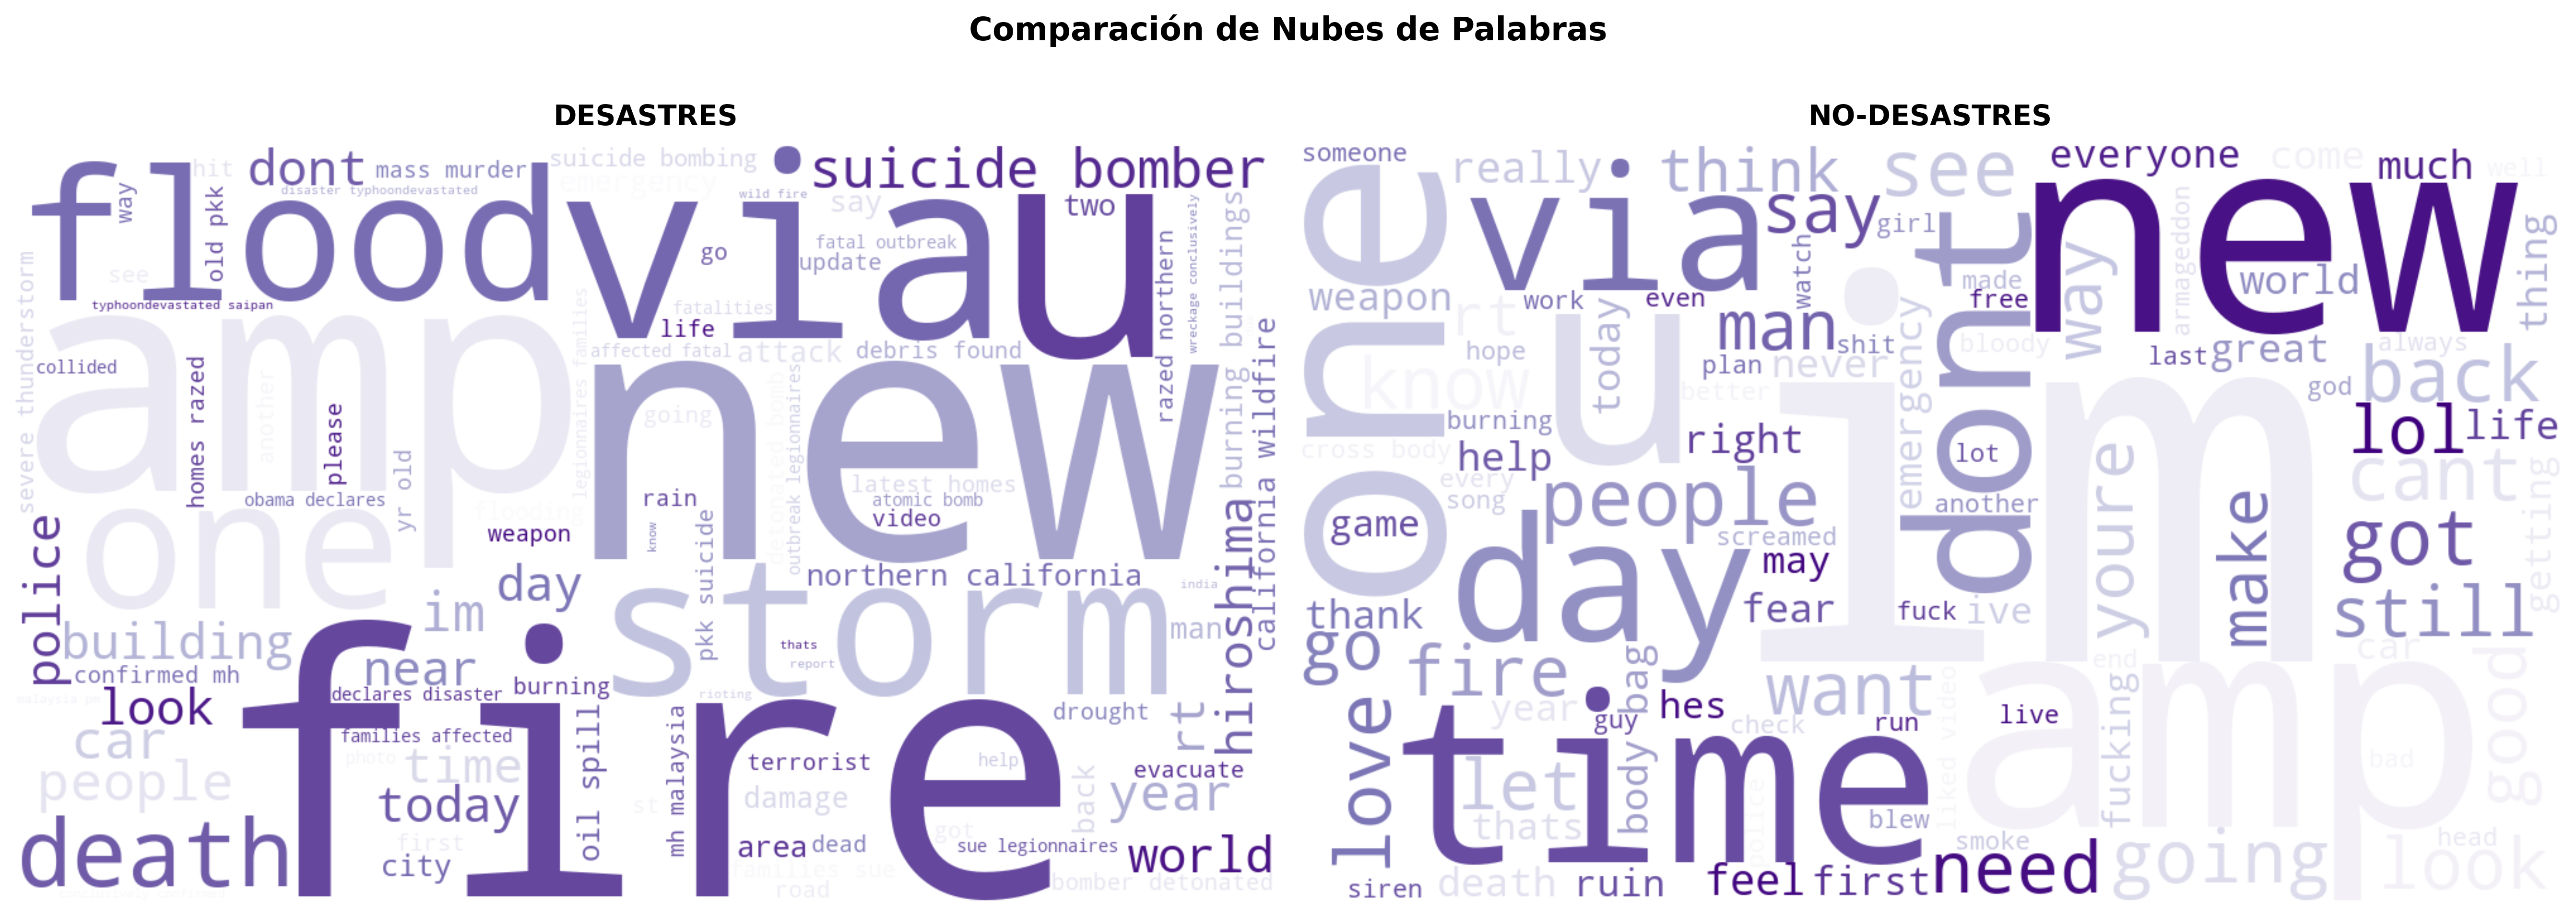
\includegraphics[width=\textwidth]{../img/wordcloud_comparacion.png}
  \caption{Nubes de palabras para tweets de desastres y no desastres.}
  \label{fig:nubes}
\end{figure}

\section{Unigramas, bigramas y trigramas}

Los n-gramas se generaron \textbf{dentro de cada tweet}. Para un tweet tokenizado como $(w_1,\dots,w_m)$, se enumeraron las ventanas consecutivas $(w_i,\dots,w_{i+n-1})$ y solo después se agregaron sus conteos por clase. Concatenar todos los tweets antes de formar ventanas habría creado secuencias inexistentes entre el final de un tweet y el inicio del siguiente.

Para cada clase $c$, la frecuencia observada fue $f_c(g)$ y la probabilidad relativa se calculó como
\[
  \widehat{P}(g\mid c)=\frac{f_c(g)}{\sum_{g'} f_c(g')}.
\]
Los conteos y estas probabilidades no recibieron suavizado. El $+1$ de Laplace se usó únicamente en ratios exploratorios entre clases,
\[
  R(g)=\frac{f_1(g)+1}{f_0(g)+1},
\]
para evitar división por cero sin presentar apariciones ficticias como conteos observados.

\begin{table}[H]
\centering
\caption{Diversidad y totales observados de n-gramas por clase.}
\label{tab:ngramas}
\begin{tabular}{@{}lrrrr@{}}
\toprule
 & \multicolumn{2}{c}{Tipos únicos} & \multicolumn{2}{c}{Total observado} \\
\cmidrule(lr){2-3}\cmidrule(l){4-5}
Tipo & Desastre & No desastre & Desastre & No desastre \\
\midrule
Unigramas & 8,006 & 10,372 & 30,342 & 36,371 \\
Bigramas & 19,041 & 26,901 & 27,071 & 32,029 \\
Trigramas & 18,153 & 24,700 & 23,810 & 27,757 \\
\bottomrule
\end{tabular}
\end{table}

La Figura~\ref{fig:riqueza-ngramas} muestra que los bigramas aumentan la variedad contextual y que los trigramas únicos disminuyen frente a los bigramas, pues numerosos tweets son cortos. Los totales observados decrecen al aumentar $n$, como corresponde cuando se respetan los límites documentales.

\begin{figure}[H]
  \centering
  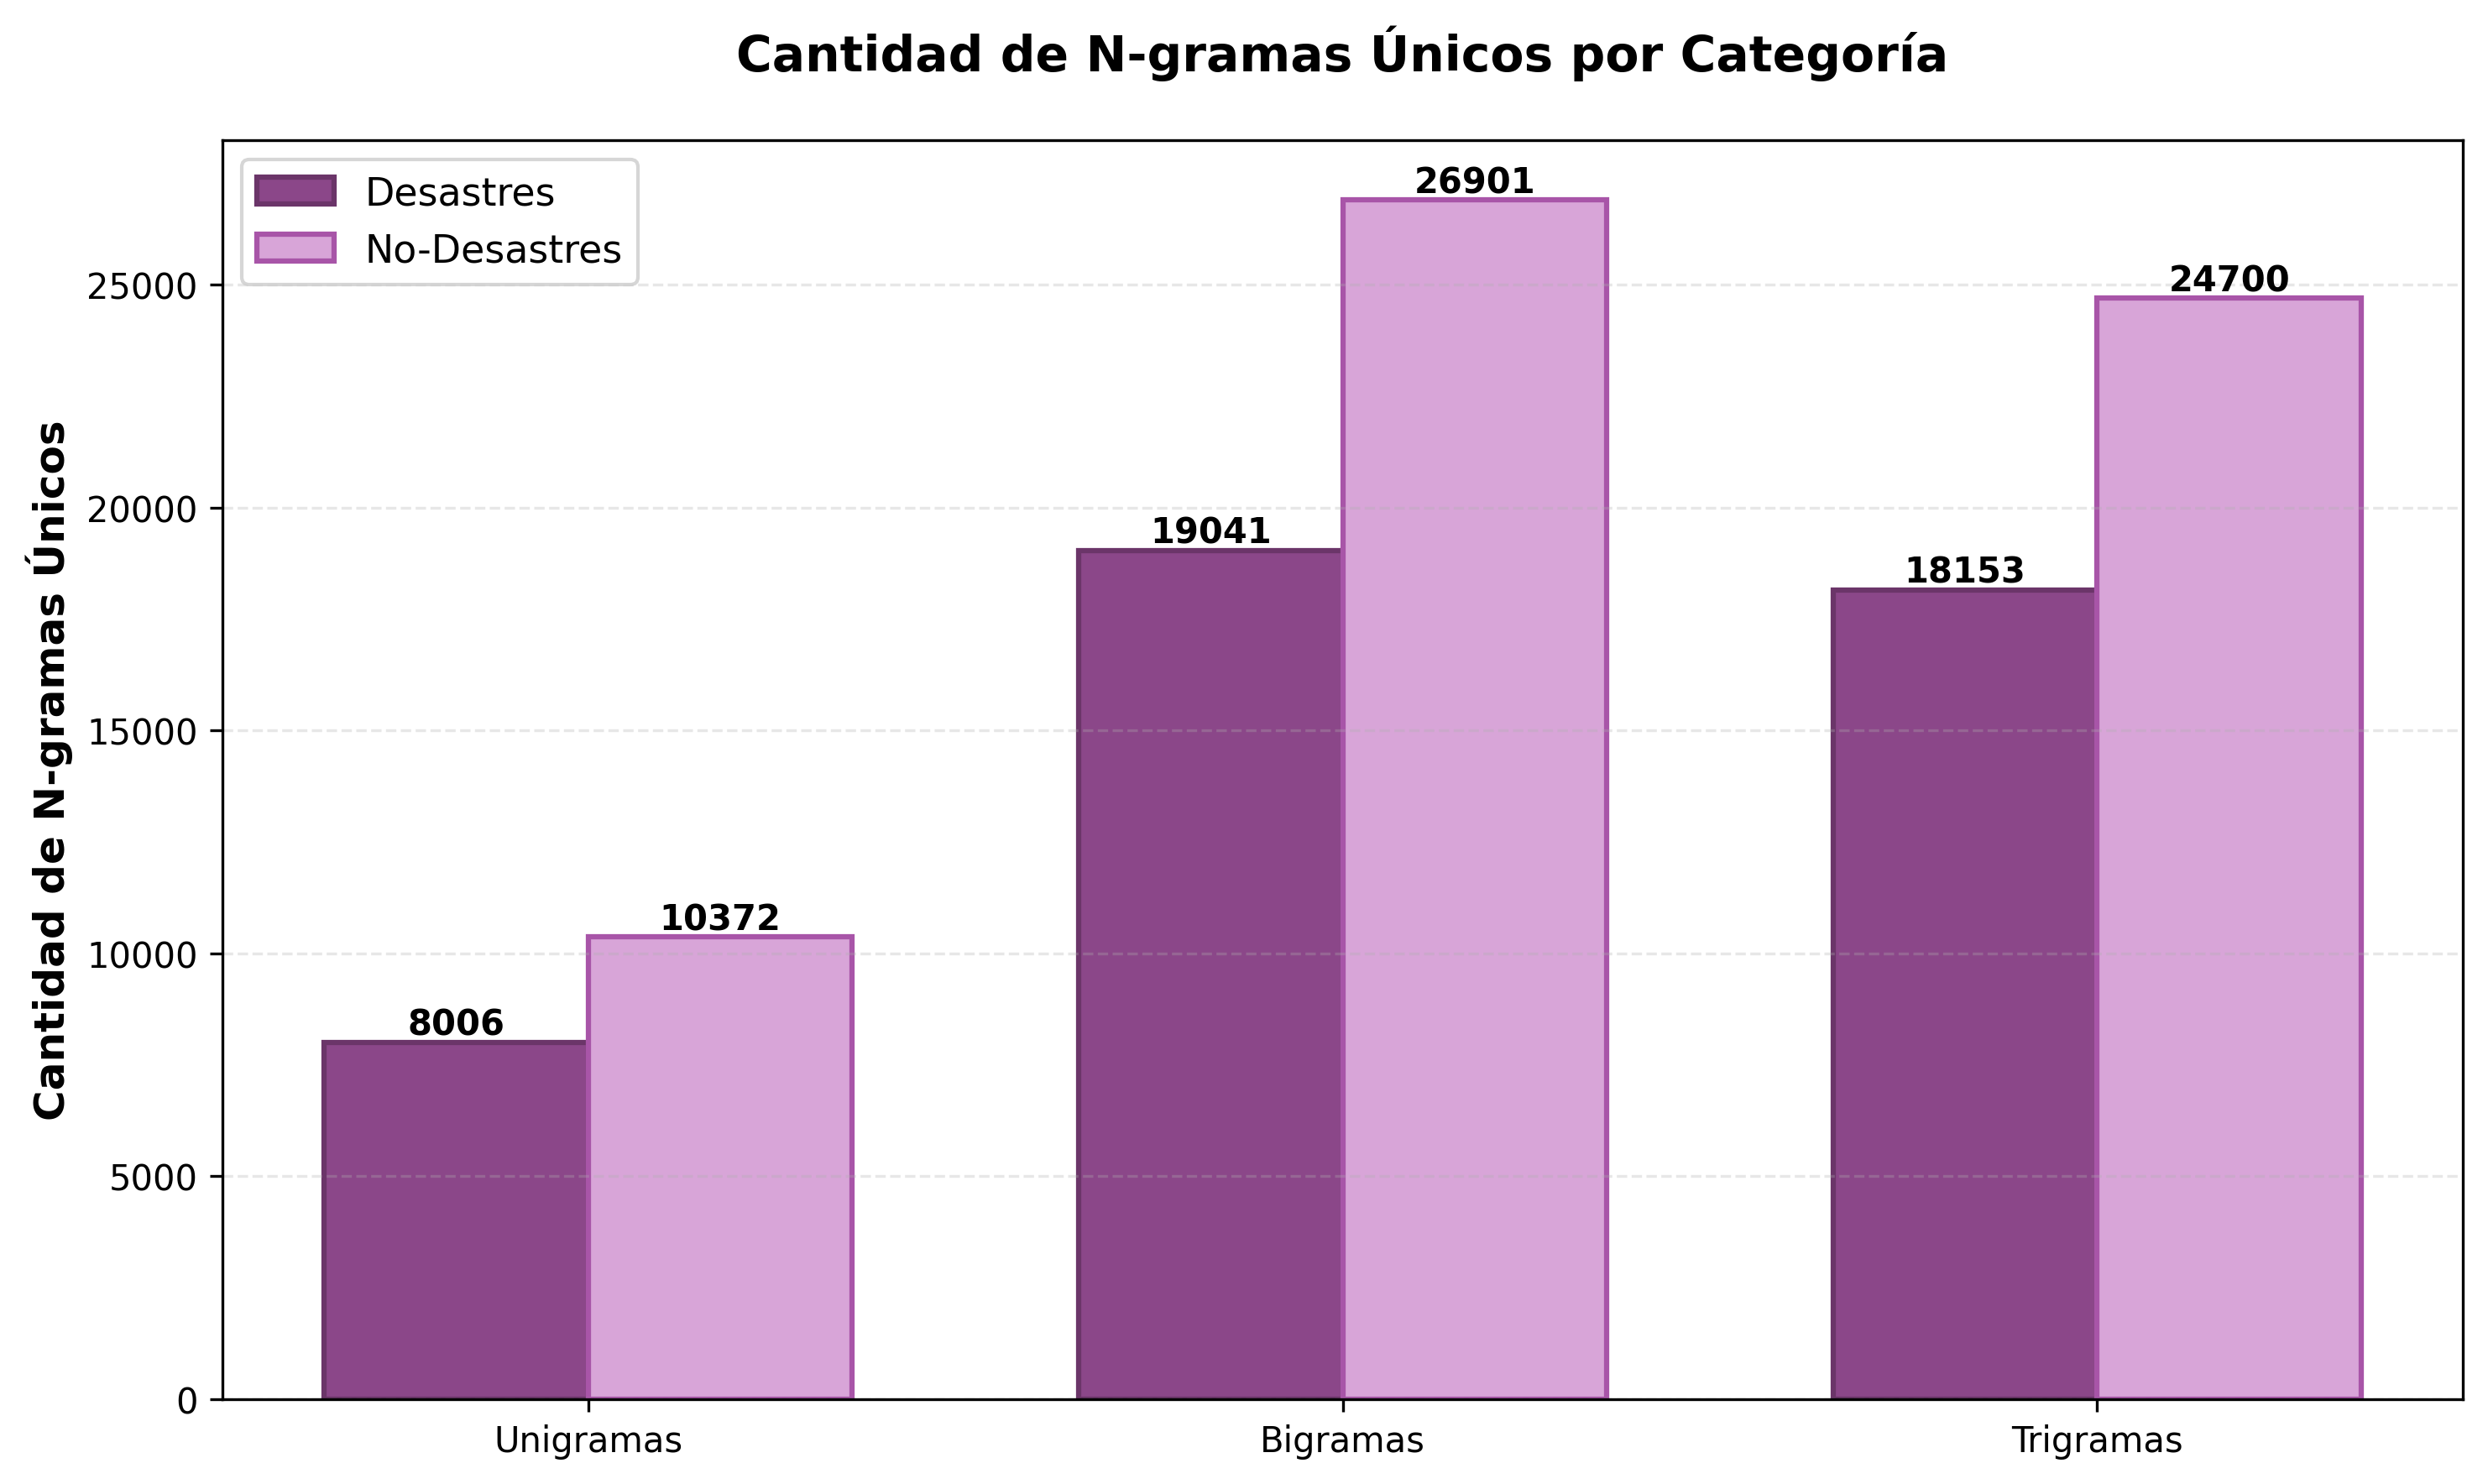
\includegraphics[width=0.8\textwidth]{../img/ngramas_cantidad.png}
  \caption{Cantidad de n-gramas únicos por categoría.}
  \label{fig:riqueza-ngramas}
\end{figure}

Entre los bigramas de desastre aparecen \emph{suicide bomber} (59), \emph{oil spill} (38), \emph{burning buildings} (35), \emph{suicide bombing} (34) y \emph{california wildfire} (34). En no desastres aparecen secuencias sobre un evento viral de Reddit y lenguaje coloquial como \emph{looks like}, \emph{feel like} y \emph{dont know}. La presencia de \emph{burning buildings} en ambas clases ilustra que el contexto ayuda, pero no elimina la ambigüedad. La comparación se presenta en la Figura~\ref{fig:bigramas}.

\begin{figure}[H]
  \centering
  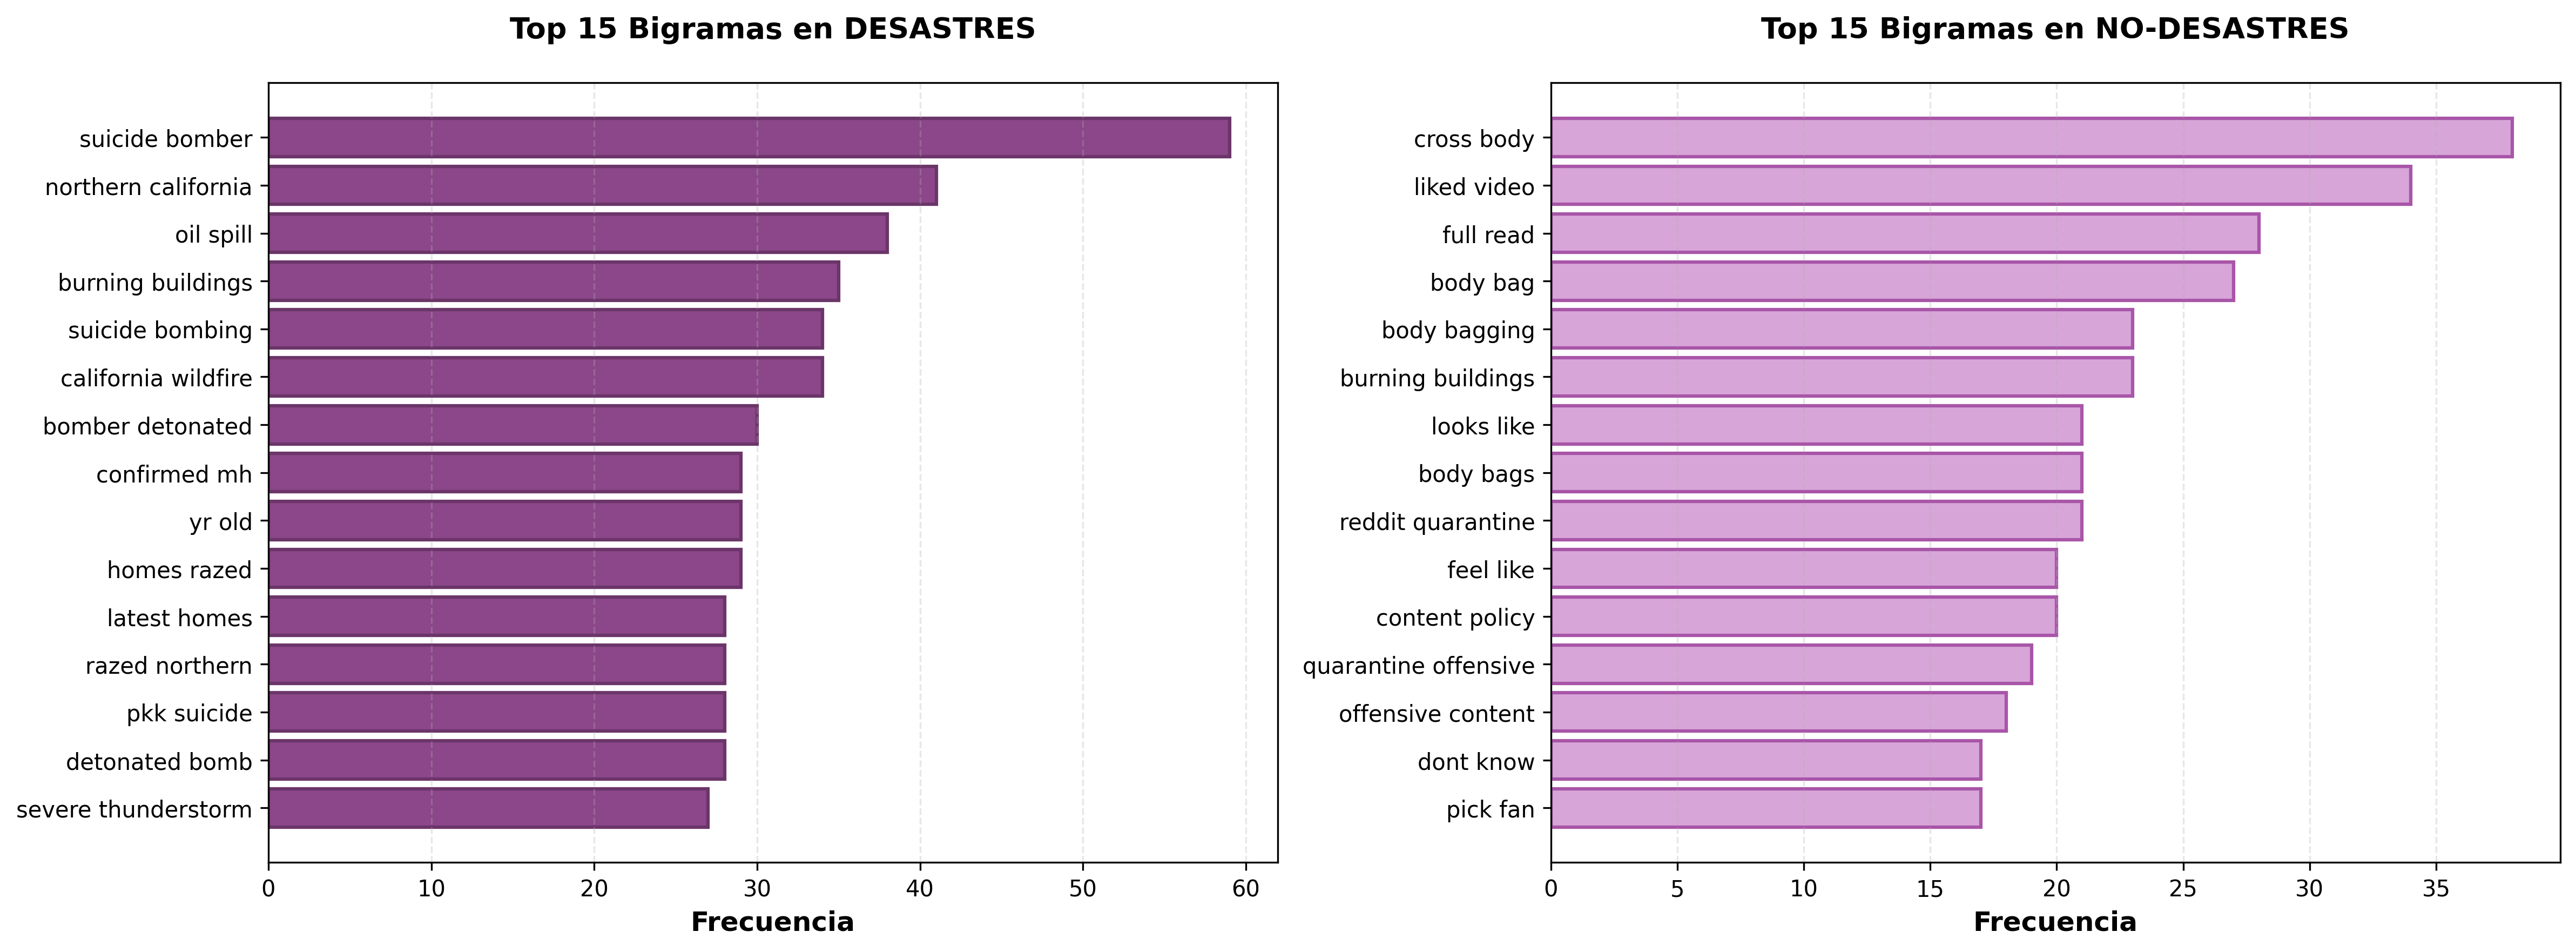
\includegraphics[width=\textwidth]{../img/bigramas_comparacion.png}
  \caption{Bigramas más frecuentes en cada categoría.}
  \label{fig:bigramas}
\end{figure}

Los trigramas aportan contexto adicional, pero varios de los más frecuentes son fragmentos de un mismo tweet viral repetido. Por tanto, su frecuencia puede representar duplicación de un evento concreto y no una regla lingüística general. Esta evidencia motivó usar unigramas y bigramas en TF--IDF: capturan contexto corto con menos dispersión y menor riesgo de memorizar cadenas extensas.

\section{Modelos de clasificación}

\subsection{Configuración}

La representación fue TF--IDF de unigramas y bigramas, limitada a 5,000 características. El vectorizador se ajustó solo con entrenamiento. Se compararon:
\begin{itemize}
  \item \textbf{Naive Bayes multinomial}: parámetros predeterminados;
  \item \textbf{regresión logística}: \code{max\_iter=1000}, \code{random\_state=42};
  \item \textbf{SVM lineal}: \code{LinearSVC(random\_state=42)}.
\end{itemize}

Las métricas consideran a desastre real como clase positiva. Exactitud resume aciertos globales; precisión cuantifica cuántas alertas positivas son correctas; \emph{recall} cuantifica cuántos desastres reales se detectan; F1 equilibra precisión y \emph{recall} \cite{sklearn,pedregosa2011}.

\begin{table}[H]
\centering
\caption{Métricas exactas del conjunto de prueba, extraídas del notebook ejecutado.}
\label{tab:modelos}
\begin{tabular}{@{}lrrrr@{}}
\toprule
Modelo & Exactitud & Precisión & Recall & F1 \\
\midrule
Naive Bayes & 0.812213 & 0.860784 & 0.671254 & 0.754296 \\
Regresión logística & \textbf{0.822718} & 0.846570 & 0.717125 & \textbf{0.776490} \\
SVM lineal & 0.795141 & 0.765528 & \textbf{0.753823} & 0.759630 \\
\bottomrule
\end{tabular}
\end{table}

La regresión logística se seleccionó por el F1 más alto. Naive Bayes fue el más preciso, pero su \emph{recall} de 0.671254 implica más desastres omitidos. SVM obtuvo el mejor \emph{recall}, a costa de una caída considerable de precisión y exactitud. La regresión logística ofrece el mejor compromiso para un problema donde importan tanto las falsas alarmas como los eventos no detectados.

\section{Función de clasificación}

La función \code{clasificar\_tweet(texto)} recibe texto crudo, ejecuta \code{limpiar\_tweet}, transforma el resultado con el vectorizador ya ajustado y aplica la regresión logística baseline. El diseño contiene una rama para concatenar VADER solo si el modelo enriquecido supera al baseline; como el experimento del Ejercicio 10 no mostró mejora, esa rama no se selecciona. La salida es ``Desastre real'' o ``No es un desastre''.

Los siguientes son outputs reales guardados en el notebook:
\begin{table}[H]
\centering
\caption{Ejemplos de ejecución de la función final.}
\label{tab:funcion}
\begin{tabularx}{\textwidth}{@{}Yl@{}}
\toprule
Tweet crudo & Salida \\
\midrule
Forest fire near La Ronge Sask. Canada & Desastre real \\
I love this weather, going to the beach today! & No es un desastre \\
BREAKING: earthquake magnitude 7.2 hits the coast, buildings collapsed & Desastre real \\
This song is fire, best track of the year & No es un desastre \\
\bottomrule
\end{tabularx}
\end{table}

Estos casos comprueban el recorrido técnico y muestran que el modelo distingue un uso literal de \emph{fire} de uno figurado. No sustituyen una evaluación externa con eventos nuevos.

\section{Sentimiento con VADER}

VADER es un modelo léxico y basado en reglas, diseñado para texto de redes sociales \cite{hutto2014}. Para cada tweet produce proporciones \code{neg}, \code{neu} y \code{pos}, además de un puntaje compuesto normalizado. Se aplicaron los umbrales convencionales: compuesto $\geq 0.05$ para positivo, $\leq -0.05$ para negativo y el intervalo intermedio para neutral \cite{nltkvader}. Al conservar el texto original, emoticones y puntuación siguen disponibles para las reglas del método.

\begin{table}[H]
\centering
\caption{Distribución exacta de sentimiento VADER.}
\label{tab:sentimiento}
\begin{tabular}{@{}lrr@{}}
\toprule
Sentimiento & Tweets & Porcentaje \\
\midrule
Negativo & 3,707 & 48.69\% \\
Neutral & 2,013 & 26.44\% \\
Positivo & 1,893 & 24.87\% \\
\midrule
Total & 7,613 & 100.00\% \\
\bottomrule
\end{tabular}
\end{table}

\section{Extremos de sentimiento y comparación por categoría}

\subsection{Diez tweets más negativos}

El orden fue determinista: mayor \code{vader\_neg}, luego menor \code{vader\_compound} y finalmente \code{id} ascendente. Debido a empates léxicos, el décimo registro no necesariamente es sustancialmente distinto del siguiente.

\small
\begin{longtable}{@{}r p{7.4cm} C{1.2cm} p{1.8cm} rr@{}}
\caption{Diez tweets con mayor negatividad VADER.}\label{tab:negativos}\\
\toprule
ID & Tweet & Target & Categoría & Neg & Comp. \\
\midrule
\endfirsthead
\multicolumn{6}{l}{\small\itshape Continuación de la Tabla~\ref{tab:negativos}}\\
\toprule
ID & Tweet & Target & Categoría & Neg & Comp. \\
\midrule
\endhead
10689 & wreck? wreck wreck wreck wreck wreck wreck wreck wreck wreck wreck wreck wreck? & 0 & No desastre & 1.000 & -0.9883 \\
5221 & Fatality! & 0 & No desastre & 1.000 & -0.6996 \\
5224 & fatality & 0 & No desastre & 1.000 & -0.6705 \\
7400 & Obliterated & 0 & No desastre & 1.000 & -0.4767 \\
2703 & Crushed & 0 & No desastre & 1.000 & -0.4215 \\
8589 & * Screams * & 0 & No desastre & 1.000 & -0.2960 \\
9106 & she's a suicide bomb & 0 & No desastre & 0.885 & -0.8271 \\
10295 & FUCK NUCLEAR WEAPON & 0 & No desastre & 0.851 & -0.6908 \\
1302 & Damn bloody hot & 0 & No desastre & 0.848 & -0.6808 \\
5259 & Fatality ???? & 0 & No desastre & 0.845 & -0.7550 \\
\bottomrule
\end{longtable}
\normalsize

Los diez extremos negativos pertenecen a \code{target=0}. Esto no contradice la comparación agregada: son casos particulares, muchos muy breves o figurativos, en los que el léxico de VADER asigna toda la masa a negatividad.

\subsection{Diez tweets más positivos}

El orden fue mayor \code{vader\_pos}, luego mayor \code{vader\_compound} y \code{id} ascendente.

\small
\begin{longtable}{@{}r p{7.4cm} C{1.2cm} p{1.8cm} rr@{}}
\caption{Diez tweets con mayor positividad VADER.}\label{tab:positivos}\\
\toprule
ID & Tweet & Target & Categoría & Pos & Comp. \\
\midrule
\endfirsthead
\multicolumn{6}{l}{\small\itshape Continuación de la Tabla~\ref{tab:positivos}}\\
\toprule
ID & Tweet & Target & Categoría & Pos & Comp. \\
\midrule
\endhead
6769 & @Benji\_Devos thanks thanks :3 & 0 & No desastre & 0.901 & 0.8442 \\
7680 & @panic awesome thanks. & 0 & No desastre & 0.875 & 0.7906 \\
8759 & Super sweet and beautiful :) \url{https://t.co/TUi9uwBvVp} & 0 & No desastre & 0.873 & 0.9300 \\
628 & @local\_arsonist LMFAO & 0 & No desastre & 0.809 & 0.6408 \\
24 & I love fruits & 0 & No desastre & 0.808 & 0.6369 \\
33 & Love skiing & 0 & No desastre & 0.808 & 0.6369 \\
935 & @Shayoly yes I love it & 0 & No desastre & 0.775 & 0.7845 \\
2486 & We're happily collided :) & 0 & No desastre & 0.767 & 0.7650 \\
40 & Cooool :) & 0 & No desastre & 0.750 & 0.4588 \\
9990 & @tsunami\_esh ESH PLEASE OKAY! & 0 & No desastre & 0.749 & 0.7147 \\
\bottomrule
\end{longtable}
\normalsize

También los diez extremos positivos pertenecen a \code{target=0}, lo que concuerda con lenguaje agradecido, afectivo o humorístico fuera de reportes reales de desastre.

\subsection{¿Los tweets de desastre son más negativos?}

La variable \code{negativity} se definió como el componente \code{neg} de VADER. Como está acotada, contiene numerosos ceros y no se asumió normalidad, se aplicó Mann--Whitney U bilateral a las dos muestras independientes \cite{mannwhitney,scipymwu}. La prueba evalúa diferencia entre distribuciones, no causalidad.

\begin{table}[H]
\centering
\caption{Resumen de negatividad por categoría.}
\label{tab:negatividad}
\begin{tabular}{@{}lrrrrrr@{}}
\toprule
Categoría & $n$ & Media & Mediana & Desv. & Q1 & Q3 \\
\midrule
Desastre real & 3,271 & 0.173582 & 0.157 & 0.167870 & 0.000 & 0.294 \\
No desastre & 4,342 & 0.132318 & 0.088 & 0.159648 & 0.000 & 0.231 \\
\bottomrule
\end{tabular}
\end{table}

El resultado fue $U=8{,}141{,}444.5$, $p=4.00854\times10^{-30}$ y efecto rango-biserial 0.1465, calculado como $2U/(n_1n_0)-1$. Existe evidencia estadística de que las distribuciones difieren y la media es mayor en desastres. Sin embargo, el tamaño de efecto es pequeño: no puede afirmarse que todo tweet de desastre sea más negativo ni que la diferencia sea grande en términos prácticos. El tamaño muestral elevado ayuda a producir un valor $p$ muy pequeño incluso ante separaciones modestas.

\section{Reentrenamiento con negatividad}

Para el Ejercicio 10, \code{negativity} es exactamente \code{vader\_neg} calculado desde el tweet original. Se reutilizaron los mismos índices del split 80/20. La matriz TF--IDF, ajustada solo con entrenamiento, se concatenó con una columna dispersa de negatividad para entrenamiento y prueba. VADER es un procedimiento fijo que no aprende del target; no se estimó ningún parámetro con el conjunto de prueba. De este modo se evitó fuga de información.

\begin{table}[H]
\centering
\caption{Regresión logística baseline frente al modelo enriquecido.}
\label{tab:neg-modelo}
\begin{tabular}{@{}lrrrr@{}}
\toprule
Configuración & Exactitud & Precisión & Recall & F1 \\
\midrule
Baseline TF--IDF & 0.822718 & 0.846570 & 0.717125 & 0.776490 \\
TF--IDF + negativity & 0.822062 & 0.847550 & 0.714067 & 0.775104 \\
\midrule
$\Delta$ (enriquecido $-$ baseline) & -0.000657 & +0.000980 & -0.003058 & -0.001386 \\
\bottomrule
\end{tabular}
\end{table}

La negatividad no mejoró el modelo. Aunque la precisión aumentó 0.000980, el \emph{recall} disminuyó 0.003058 y el F1 pasó de 0.776490 a 0.775104. La reducción de 0.001386 equivale aproximadamente a 0.14 puntos porcentuales. Por el criterio definido antes del experimento, se conserva el baseline.

\section{Limitaciones}

\begin{itemize}
  \item \textbf{Duplicados y casi duplicados.} En el CSV analizado existen 110 repeticiones exactas de \code{text} después de la primera aparición y 817 repeticiones de \code{text\_cleaned}. Estas últimas incluyen textos distintos que colapsan a la misma forma normalizada. Un split aleatorio puede colocar mensajes iguales o casi iguales en ambos subconjuntos y sobreestimar generalización.
  \item \textbf{Eventos específicos.} Palabras y trigramas frecuentes reflejan noticias virales concretas. El modelo puede memorizar eventos, personas o lugares en vez de aprender señales transferibles a futuros desastres.
  \item \textbf{Variables poco explotadas.} \code{keyword} y \code{location} no se incorporaron al clasificador. La ubicación tiene muchos nulos y formato libre, pero ambas variables podrían aportar información con codificación y validación cuidadosas.
  \item \textbf{Alcance de VADER.} Es un recurso general para redes sociales en inglés; puede fallar ante sarcasmo, jerga, lenguaje noticioso neutral, ambigüedad y nombres propios.
  \item \textbf{Sesgo del conjunto.} Los tweets corresponden a una selección y periodo concretos de la competencia; clase, idioma, plataforma y tópicos no representan necesariamente otros contextos.
  \item \textbf{Significancia frente a relevancia.} El valor $p$ muy pequeño no implica un efecto grande. El rango-biserial de 0.1465 y la falta de mejora del F1 muestran que la diferencia afectiva tiene utilidad predictiva limitada en esta configuración.
  \item \textbf{Selección y evaluación.} Los modelos se compararon en un único conjunto de prueba. Una estimación más rigurosa requeriría validación cruzada para selección y un conjunto final independiente, idealmente separado por evento o por tiempo.
\end{itemize}

\section{Conclusiones}

\begin{enumerate}
  \item \textbf{¿Qué vocabulario ayuda a clasificar?} Los términos de incidentes concretos y sus combinaciones cortas son informativos, mientras que palabras compartidas como \emph{via}, \emph{amp} o \emph{people} discriminan poco de forma aislada. Los ratios entre clases son útiles para explorar, pero deben interpretarse con cautela ante términos raros y tweets repetidos.
  \item \textbf{¿Vale la pena explorar bigramas y trigramas?} Sí. Los bigramas recuperan contexto que los unigramas pierden y justifican TF--IDF 1--2. Los trigramas revelan cadenas de eventos y duplicación, pero son más dispersos y propensos a memorizar tweets virales; por ello no se incorporaron al modelo final.
  \item \textbf{¿Cuál clasificador se debe conservar?} La regresión logística baseline, porque obtuvo el mayor F1 (0.776490) y el mejor compromiso entre precisión y \emph{recall} en el split común.
  \item \textbf{¿Los tweets de desastre son más negativos?} En promedio y distribución, sí existe una diferencia estadística: 0.173582 frente a 0.132318 y $p=4.00854\times10^{-30}$. La respuesta práctica debe ser prudente, pues el efecto 0.1465 es pequeño y los extremos individuales no siguen necesariamente la tendencia agregada.
  \item \textbf{¿La negatividad mejoró la clasificación?} No. El F1 disminuyó 0.001386 y el \emph{recall} también cayó. La señal afectiva existe a nivel grupal, pero está parcialmente contenida en el vocabulario o es demasiado débil y ambigua para aportar al baseline de esta prueba.
  \item \textbf{¿La función satisface el objetivo operativo?} Sí: recibe un tweet crudo, reproduce la limpieza y vectorización del entrenamiento y devuelve una categoría. Su uso fuera del conjunto debe acompañarse de monitoreo y evaluación con eventos no vistos.
\end{enumerate}

\clearpage
\appendix
\section{Reproducibilidad}

Desde la raíz del repositorio:
\begin{verbatim}
uv sync --locked
uv run jupyter lab Lab5_Completo.ipynb
\end{verbatim}

El notebook verifica y descarga los recursos de NLTK cuando son necesarios. Una descarga explícita equivalente es:
\begin{verbatim}
uv run python -m nltk.downloader stopwords vader_lexicon
\end{verbatim}

Para ejecutar todas las celdas y actualizar sus outputs:
\begin{verbatim}
uv run jupyter nbconvert --to notebook --execute --inplace \
  Lab5_Completo.ipynb
\end{verbatim}

Para compilar este informe desde \code{report/}:
\begin{verbatim}
/usr/bin/pdflatex -interaction=nonstopmode \
  -jobname=Laboratorio_5_Informe lab5_report.tex
/usr/bin/pdflatex -interaction=nonstopmode \
  -jobname=Laboratorio_5_Informe lab5_report.tex
\end{verbatim}

El informe de trabajo y el repositorio están disponibles en \url{https://github.com/Qu3zada22/lab5-ds}. Este repositorio contiene el código, el notebook, la fuente LaTeX y el PDF compilado.

\clearpage
\begin{thebibliography}{99}

\bibitem{kaggle}
Kaggle. \emph{Natural Language Processing with Disaster Tweets}. Datos de la competencia. Disponible en: \url{https://www.kaggle.com/competitions/nlp-getting-started/data}. Consultado el 29 de agosto de 2026.

\bibitem{hutto2014}
Hutto, C. J. y Gilbert, E. (2014). VADER: A Parsimonious Rule-Based Model for Sentiment Analysis of Social Media Text. \emph{Proceedings of the International AAAI Conference on Web and Social Media}, 8(1), 216--225. \url{https://doi.org/10.1609/icwsm.v8i1.14550}.

\bibitem{nltkvader}
NLTK Project. \emph{NLTK Sentiment VADER API documentation}. Disponible en: \url{https://www.nltk.org/api/nltk.sentiment.vader.html}. Consultado el 29 de agosto de 2026.

\bibitem{pedregosa2011}
Pedregosa, F. et al. (2011). Scikit-learn: Machine Learning in Python. \emph{Journal of Machine Learning Research}, 12, 2825--2830. Disponible en: \url{https://jmlr.org/papers/v12/pedregosa11a.html}.

\bibitem{sklearn}
Scikit-learn developers. \emph{Scikit-learn documentation}. Disponible en: \url{https://scikit-learn.org/stable/}. Consultado el 29 de agosto de 2026.

\bibitem{scipymwu}
SciPy community. \emph{scipy.stats.mannwhitneyu documentation}. Disponible en: \url{https://docs.scipy.org/doc/scipy/reference/generated/scipy.stats.mannwhitneyu.html}. Consultado el 29 de agosto de 2026.

\bibitem{mannwhitney}
Mann, H. B. y Whitney, D. R. (1947). On a Test of Whether One of Two Random Variables Is Stochastically Larger than the Other. \emph{The Annals of Mathematical Statistics}, 18(1), 50--60. \url{https://doi.org/10.1214/aoms/1177730491}.

\bibitem{scipy}
Virtanen, P. et al. (2020). SciPy 1.0: Fundamental Algorithms for Scientific Computing in Python. \emph{Nature Methods}, 17, 261--272. \url{https://doi.org/10.1038/s41592-019-0686-2}.

\bibitem{jurafsky}
Jurafsky, D. y Martin, J. H. \emph{Speech and Language Processing}, 3.a ed., borrador en línea. Disponible en: \url{https://web.stanford.edu/~jurafsky/slp3/}. Consultado el 29 de agosto de 2026.

\bibitem{jurafskyngrams}
Jurafsky, D. y Martin, J. H. \emph{N-grams}, material de \emph{Speech and Language Processing}. Disponible en: \url{https://lagunita.stanford.edu/c4x/Engineering/CS-224N/asset/slp4.pdf}.

\bibitem{feinerer2008}
Feinerer, I., Hornik, K. y Meyer, D. (2008). Text Mining Infrastructure in R. \emph{Journal of Statistical Software}, 25(5), 1--54. \url{https://doi.org/10.18637/jss.v025.i05}.

\end{thebibliography}

\end{document}
